\newpage
\section{2 Dimensional Analysis}
This section will discuss the trend and effect of various undertray variables in 2 dimensions. The variables tested consist of inlet angle \& diffuser angle which the optimised value will be used as a preliminary variable in 3 dimensional undertray design. The 2D analysis will consist of Enclosed flow analysis which use the Venturi-tube like geometry to simulate the flow of the undertray, and open-flow analysis used the bluff body to simulate the flow behaviour as well the interaction between the undertray and the bluff body. 

\subsection{2D Enclosed Flow}
\subsubsection{Overview}
2D Enclosed flow analysis serve a purpose in creating fundamental understanding of the undertray flow physics. Diffuser and inlet angle was chosen to be the main variables which fundamentally known to affect the undertray's performance. It is so called 'Enclosed' due to its geometry which shaped like a half venturi meter which cap the analysis to only the lower part of the undertray without considering any surrounding flow ahead and behind the car it self.  %try to reference every paper which have the diffuser and inlet analysis %also reference the FSUK rules

\subsubsection{Geometry and Mesh Generation}
\noindent The general geometry of this analysis is illustrated on figure \ref{fig:2D_EN_Geom} below. A realistic preliminary dimension was chosen to obtain a general picture of the undertray shape in 2D. The geometry represents the underside of the car which consist of undertray (top-wall), moving-floor (bottom-wall), velocity-inlet (left), and outlet (right). At this stage, the length of the car was generalised to be 2000 mm, with 200 mm inlet and 600 mm diffuser horizontal length. Gap clearance (the minimum distance between the undertray and the floor) has been chosen to be 30 mm which comply the minimum gap clearance distance rules of FSUK. Geometry of undertrays was generated in 2 variable forms; the first form is the increase of diffuser angle from 10 to 20 degrees in the increments of 2 degrees, and accompanied with 10 degrees inlet angle for every geometry. The second form is the increase of inlet angle from 10 to 20 degrees in the increments of 2 degrees, and accompanied with 10 degrees diffuser angle for every geometry. This format allows a preliminary development in understanding the effect of both undertray's outlet and inlet angle in isolated flow-field. 

\begin{figure}[!ht]
    \centering
    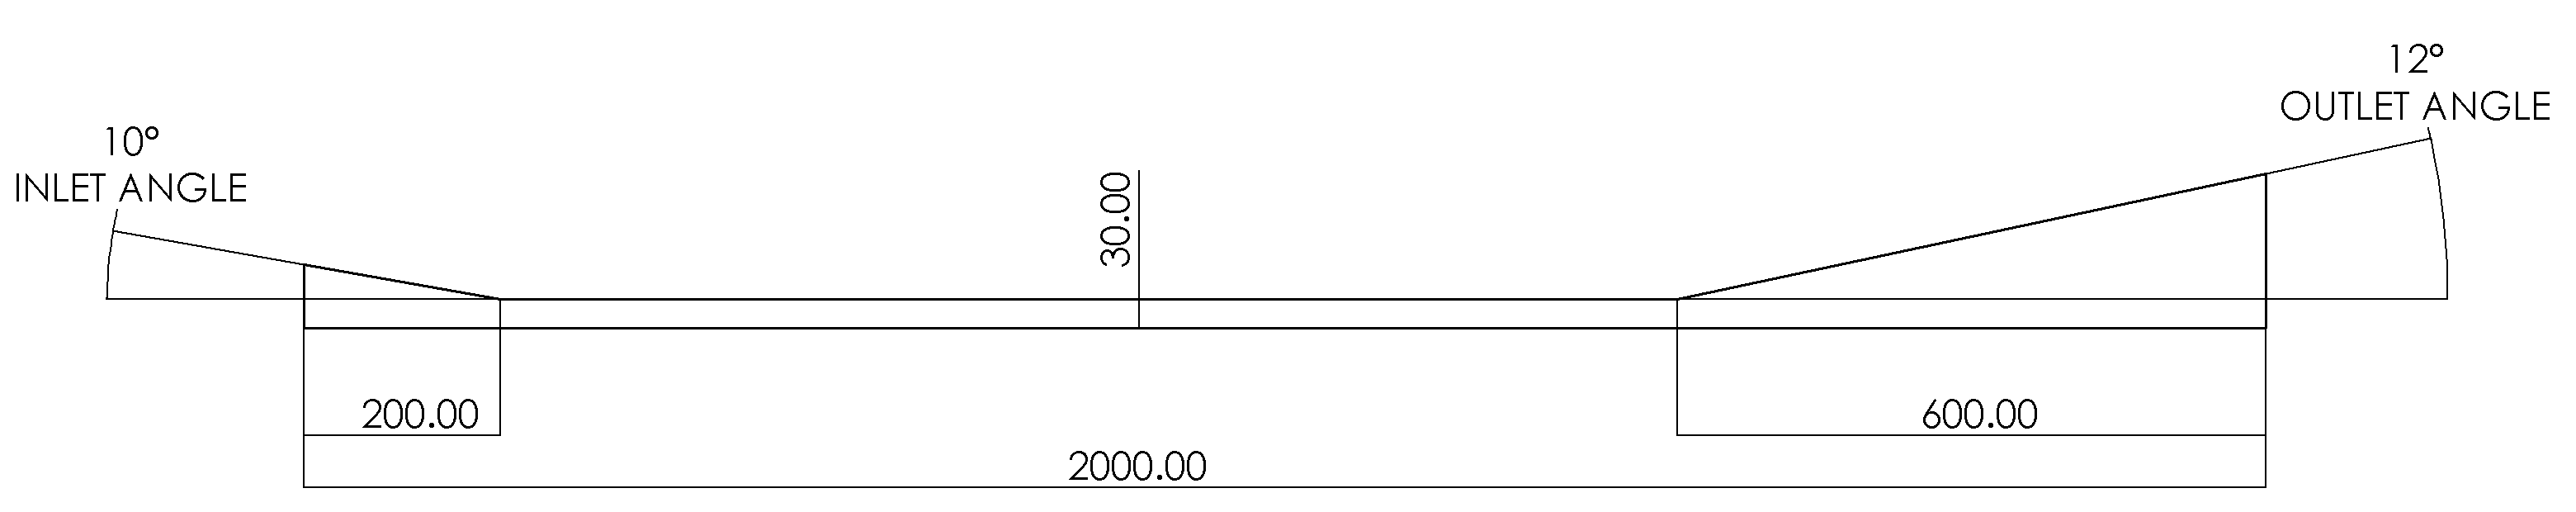
\includegraphics[scale=0.18]{Figures/2D_EN/2D_EN_D.PNG}
    \caption{2D Enclosed Geometry}
    \label{fig:2D_EN_Geom}
\end{figure}
  
\noindent A structured quadrilateral mesh was generated and inflation layer was initialised on the underside of the undertray. 20 layers of inflation with value of y$^+$ = 1 which gives the first layer distance of 2.24x$10^{-5}$ meters. Generally, the mesh element generated for each geometry in 2D Enclosed Flow analysis is around 20000 to 25000 elements depending on the variable. The quality of the mesh produced is considerably good with skewness average of 3.67x$10^{-2}$ and aspect ratio average of 31 which slightly above the range of recommendation \cite{Lanfrit2005BestFLUENT}, however, convergence criterion is still met. Figure \ref{fig:2D_EN_MESH} in appendix A shows a mesh generated from one of the 2D enclosed geometries with inflation layer details.

\subsubsection{Results \& Discussion}
Results of this analysis will be discussed on the basis of how changes in outlet and inlet angle affected the downforce (negative lift) and drag of the undertray. Figure \ref{fig:2D_EN_result} depicts plotted lift and drag of the simulations for both variables and turbulence models. Figure \ref{fig:2D_EN_result} left shows the trend of undertray's lift and drag with changes of diffuser angle variable and the inlet angle variable on the right. 

\noindent k-epsilon and k-omega turbulence model were employed in this analysis as recommended\cite{} and discussed in section(). As shows on figure \ref{fig:2D_EN_result} below, a similar trend emerged for both turbulence model. There are no significant difference on both numerical method, however,  some anomalies occurred on some of the results. For instance, both k-omega lift in 16 degree diffuser and inlet angle, and the k-omega drag at 20 degree inlet angle are considered to be a little higher than the trend pattern. Nonetheless, pattern from both variables are clear, and can be used as a preliminary understanding of the undertray.

\begin{figure}[!ht]
  \noindent
  \makebox[\textwidth]{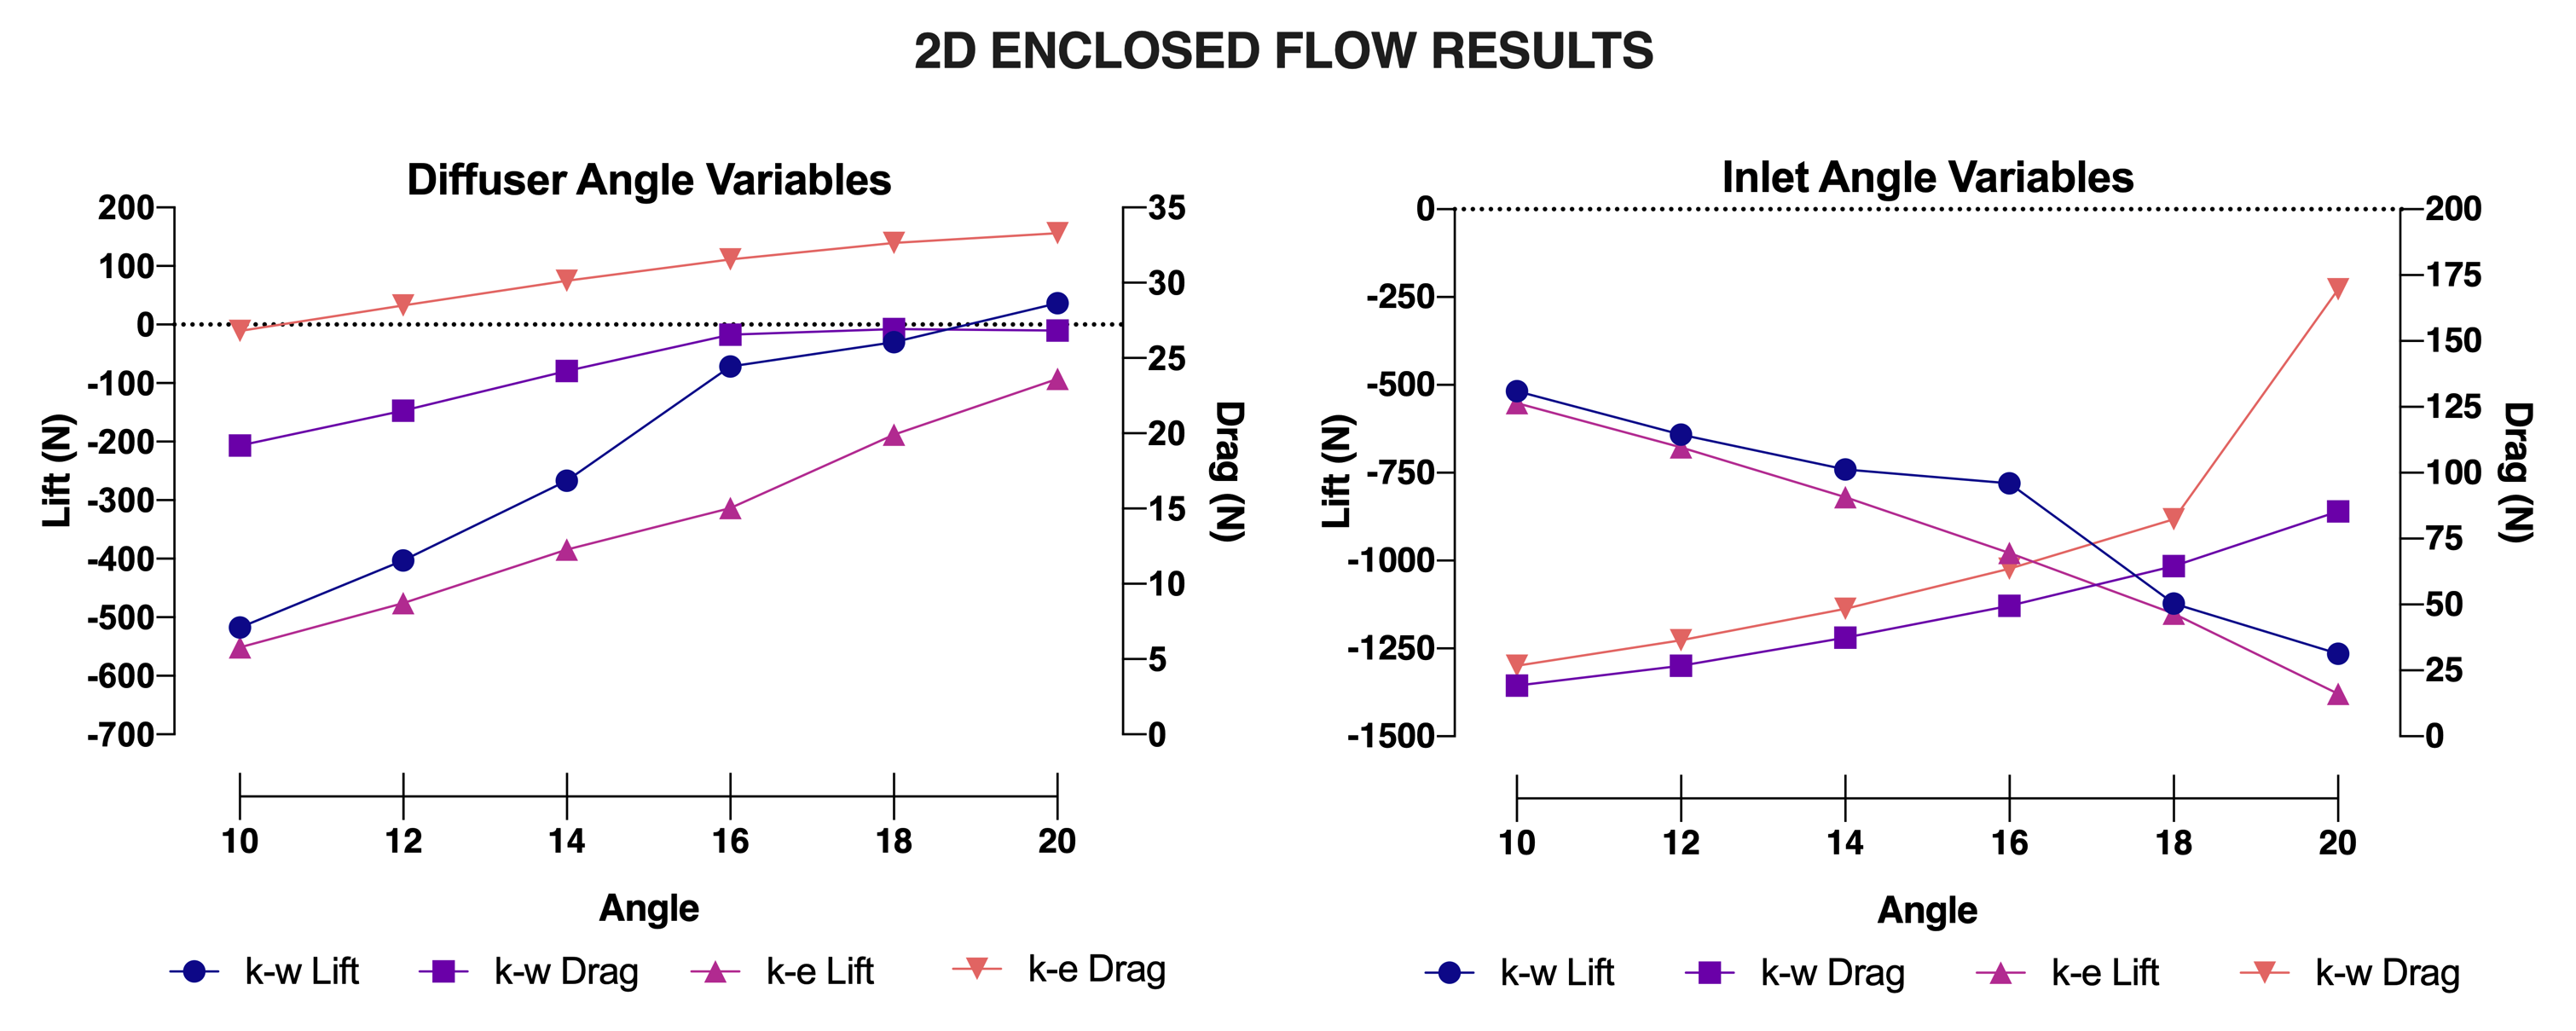
\includegraphics[scale=0.65]{Figures/2D_EN/2D_EN.png}}
  \caption{Lift and drag plot of 2D Enclosed flow analysis trend for both diffuser (left) and inlet (right) angle variables. }
  \label{fig:2D_EN_result}
\end{figure}

\noindent The main goal of a diffuser is to slowly expand the accelerated flow from the undertray's throat which acts as a pressure and flow recovery system of an undertray. An efficient diffuser allows slow pressure recovery which indicated by the flow attachment throughout the diffuser's wall. However, the diffuser angle variable plot on \textbf{figure \ref{fig:2D_EN_result}} left shows a linear degradation in the undertray's performance. The plot trend shows an increase in diffuser angle that directly proportional to the undertray's lift and drag, this is generally due to an early flow separation on the transition region between the undertray's throat and diffuser region. 

\noindent Sharp corner and high velocity are the main issue which detach the flow early and create a sudden pressure changes. Figure \ref{fig:2D_EN_streamline_compare} shows the velocity streamline from both 10 degree and 20 degree diffuser angle. The figure shows similar separation point of the streamline when the flow enters the diffuser region, this phenomenon is more obvious on the larger diffuser angle (fig \ref{fig:2D_EN_streamline_compare} (right)) as low pressure region formed which indicated in dark blue colour. Linear increase in drag is explained by the low pressure region formed on the diffuser area which acts as a vacuum which pull the undertray contrary to its direction.  

\begin{figure}[!h]
    \centering
    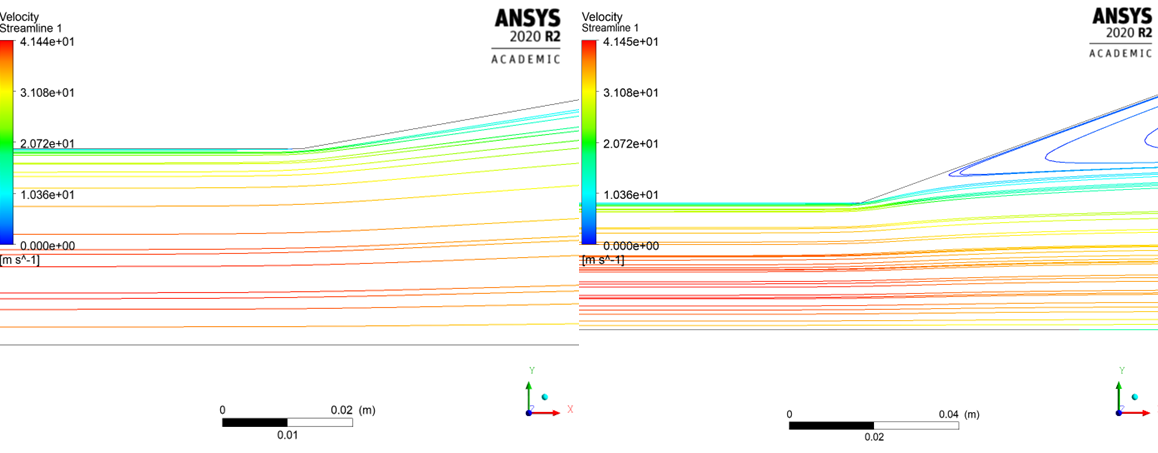
\includegraphics[height= 6cm]{Figures/2D_EN/2D_EN_Streamline_compare.PNG}
    \caption{Undertray's velocity streamline for 10 degree (left) and 20 degree (right) diffuser angle.}
    \label{fig:2D_EN_streamline_compare}
\end{figure}


\noindent From \textbf{figure \ref{fig:wall_shear_plot_2D_EN} left} in \textbf{Appendix A} ,  it can be observed that flow detachment occurred at an identical point of the undertray at any given diffuser angle which indicated by a similar pattern of second peak on the graph. Moreover,  flow detachment also occurred due to the adverse pressure gradient which is indicated on the second lower peak on the static pressure plot in figure \ref{fig:pressure_plot_2D_EN} \textbf{Appendix A}.

\noindent On the other hand, the inlet angle variable has a contrary result than previous variable. \textbf{Figure \ref{fig:2D_EN_result}} right shows that the lift  is inversely proportional to the drag as the inlet angle increases.  As the cross section area on the inlet nozzle converging, the flow is forced to convert the pressure energy into kinetic energy indicated by the increase its velocity which then drops the pressure in the undertray's throat. This condition creates a lower pressure region on the undertray's throat, hence increasing the downforce.This phenomena obeys the Bernoulli formula\textbf{ (equation \ref{eq:bernoulli})} where pressure and cross-sectional area is inversely proportional to the flow's velocity, assuming the flow in the inlet region are steady and incompressible.  Elevation in inlet angle also provide more tangential surface to be imposed by the incoming flow, this create a higher shear stress on the inlet wall and increase the overall drag. This condition also indicated on the first peak of the wall shear on figure \ref{fig:wall_shear_plot_2D_EN} left which shows a significant increase in shear stress at the corner between inlet and throat region.

\noindent Further analysis of wall shear stress \textbf{(figure \ref{fig:wall_shear_plot_2D_EN} (right))} and static pressure \textbf{(figure \ref{fig:pressure_plot_2D_EN} (right))} plot for inlet angle variables in \textbf{appendix A} shows a general increase in shear stress with inlet angle elevation accompanied by the overall pressure drop as the angle increases. This explains increase in total downforce with the elevation of inlet angle.



%%%%%%%%%%%%%%%%%%%%%%%%%%%%%
%%% 2D OPEN FLOW ANALYSIS %%%
%%%%%%%%%%%%%%%%%%%%%%%%%%%%%


\subsection{2D Open-Flow}
\subsubsection{Overview}
Previous analysis provides fundamental understanding of how changes in inlet and diffuser angle may affect its overall performance and it solely focused on the internal flow of the undertray without taking an account of the flow surrounding it. This section will be an extension of the previous analysis which to understand the effect of similar variable with additional bluff body added to the geometry. 

\subsubsection{Geometry and Mesh Generation}
This section will utilise multiple type of bluff body will be used to simulate the flow behaviour around the body and how it will affect the general performance of an undertray. Four different geometries was built on generative decision which each serve its own purpose in this analysis. A rough calculation of QFR car's length was initiated. Geometry 1,2, \& 3 has 2.6 meters of undertray length with similar inlet and diffuser configuration as previous analysis. However, Geometry 4 has a slightly different undertray configuration; with 2.85 meters of length, 1 meters smooth rounded diffuser, and 0.25 meters of inlet angle. Worth noting that the code 'A' stands for 'analysis' which indicates type of geometry used in the discussions and figures.

\begin{figure}[!ht]
    \centering
    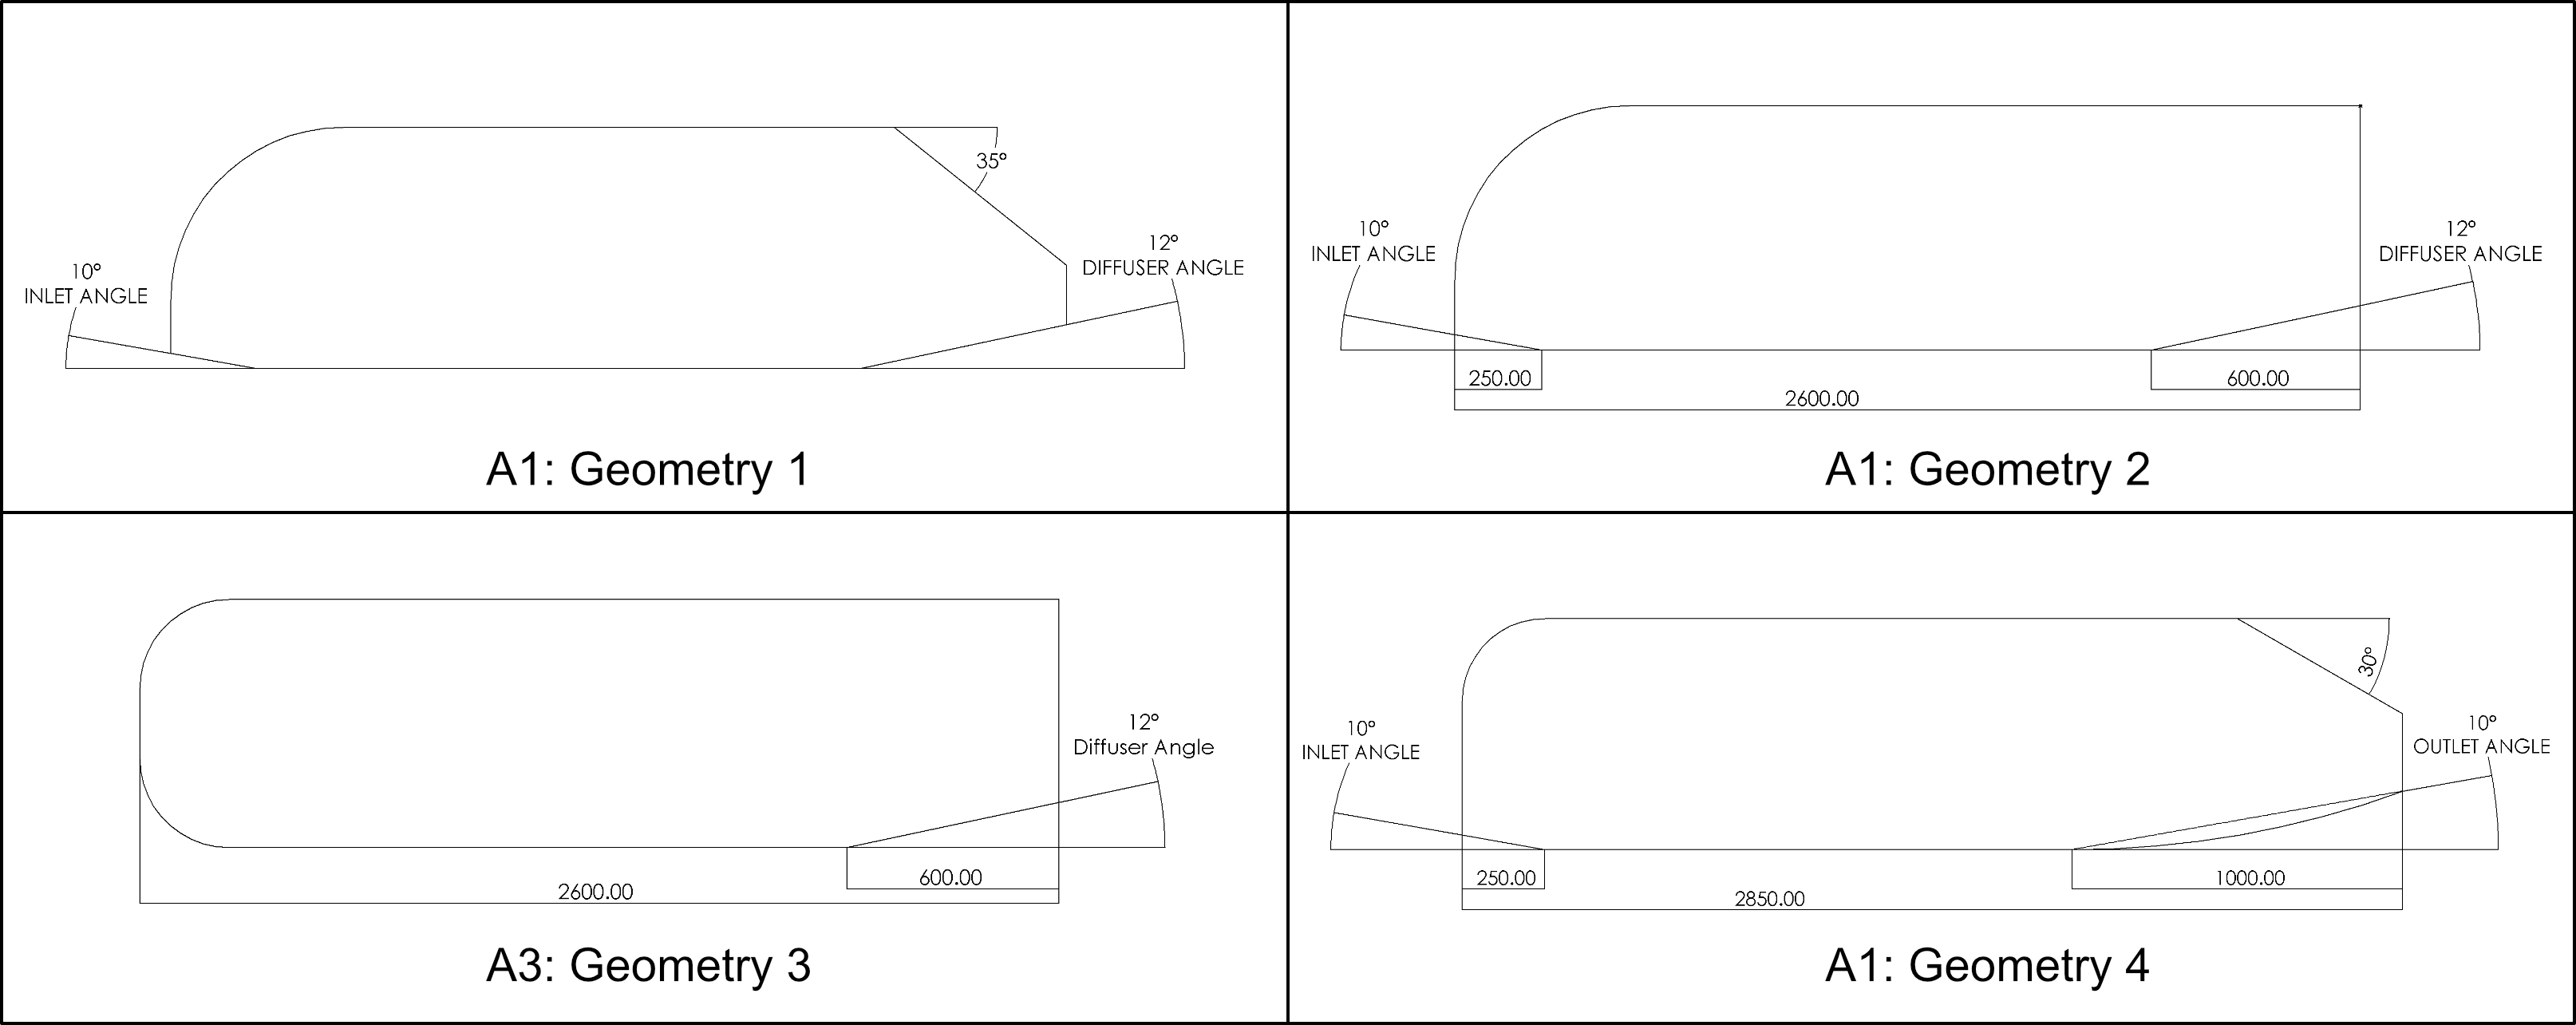
\includegraphics[scale = 0.58]{Figures/2D_OF/2D_OF_GEOM.png}
    \caption{Four geometries generated for 2D open-flow analysis.}
    \label{fig:2D_OF_GEOM}
\end{figure}
\noindent The geometry can be grouped into 2 categories. The first category consist of A1, A2, \& A3, which focus on how the geometry of the bluff body sculpt the surrounding flow and affect the overall performance of the undertray. First geometry acts as the baseline model with a 35 degree slant angle at the rear body to simulate the flow separation that also occurs at rear of QFR car. Similar to geometry 1, the second geometry has a similar dimension without inlet angle and the slant angle with purpose of simulating an immediate separation at the rear. Geometry 3 has a similar configuration as geometry 2 with no inlet elevation and filleted corner in inlet region to provide a smooth flow at intake.

\noindent Second category consist of geometry 4 which is the regeneration due to the result from previous analysis.

This geometry used a curved diffuser configuration where one end is tangential to the throat. A construction line was made between two point of the diffuser as an angle reference point from the horizontal axis. In diffuser variable analysis, a rounded inlet such as geometry 3 without any elevation was used. The purpose of such rounded inlet and diffuser was initially surmised to allow smooth intake and slows flow separation in the diffuser region due to the sharp transition from previous analyses. A Slant angle of 35 degree was also decided to be utilised to provide geometric similarity to the QFR car.

\noindent A hybrid mesh was generated for this analysis. This consist of unstructured triangular and quadrilateral mesh (or inflation) near the bluff body and the floor to identify the effect of boundary layer interaction between the undertray and floor wall.  Detailed graphics of 2D open-flow mesh can be seen on \textbf{figure \ref{fig:2D_OF_MESH}} in \textbf{appendix B}.
%add details average of the mesh quality criterion (mesh number, AR, skewness, quality)



\subsubsection{Results \& Discussion}

\noindent A 2D computational simulations have been done and the results shown will be based on the downforce and drag of the entire bluff body. Analysis 1 and 2 has a geometric similarity apart from the slant angle. The first part of the discussion will focus on how slant angle affect the flow at the rear and it impacts the undertray's performance. Figure \ref{fig:2D_OF_A12_results} below depicts the variations in trend in downforce (left) for both diffuser and inlet angle. The variations of lift and drag due to the inlet angle also shown on figure \ref{fig:2D_OF_A12_results} (right).

\begin{figure}[!ht]
    \centering
    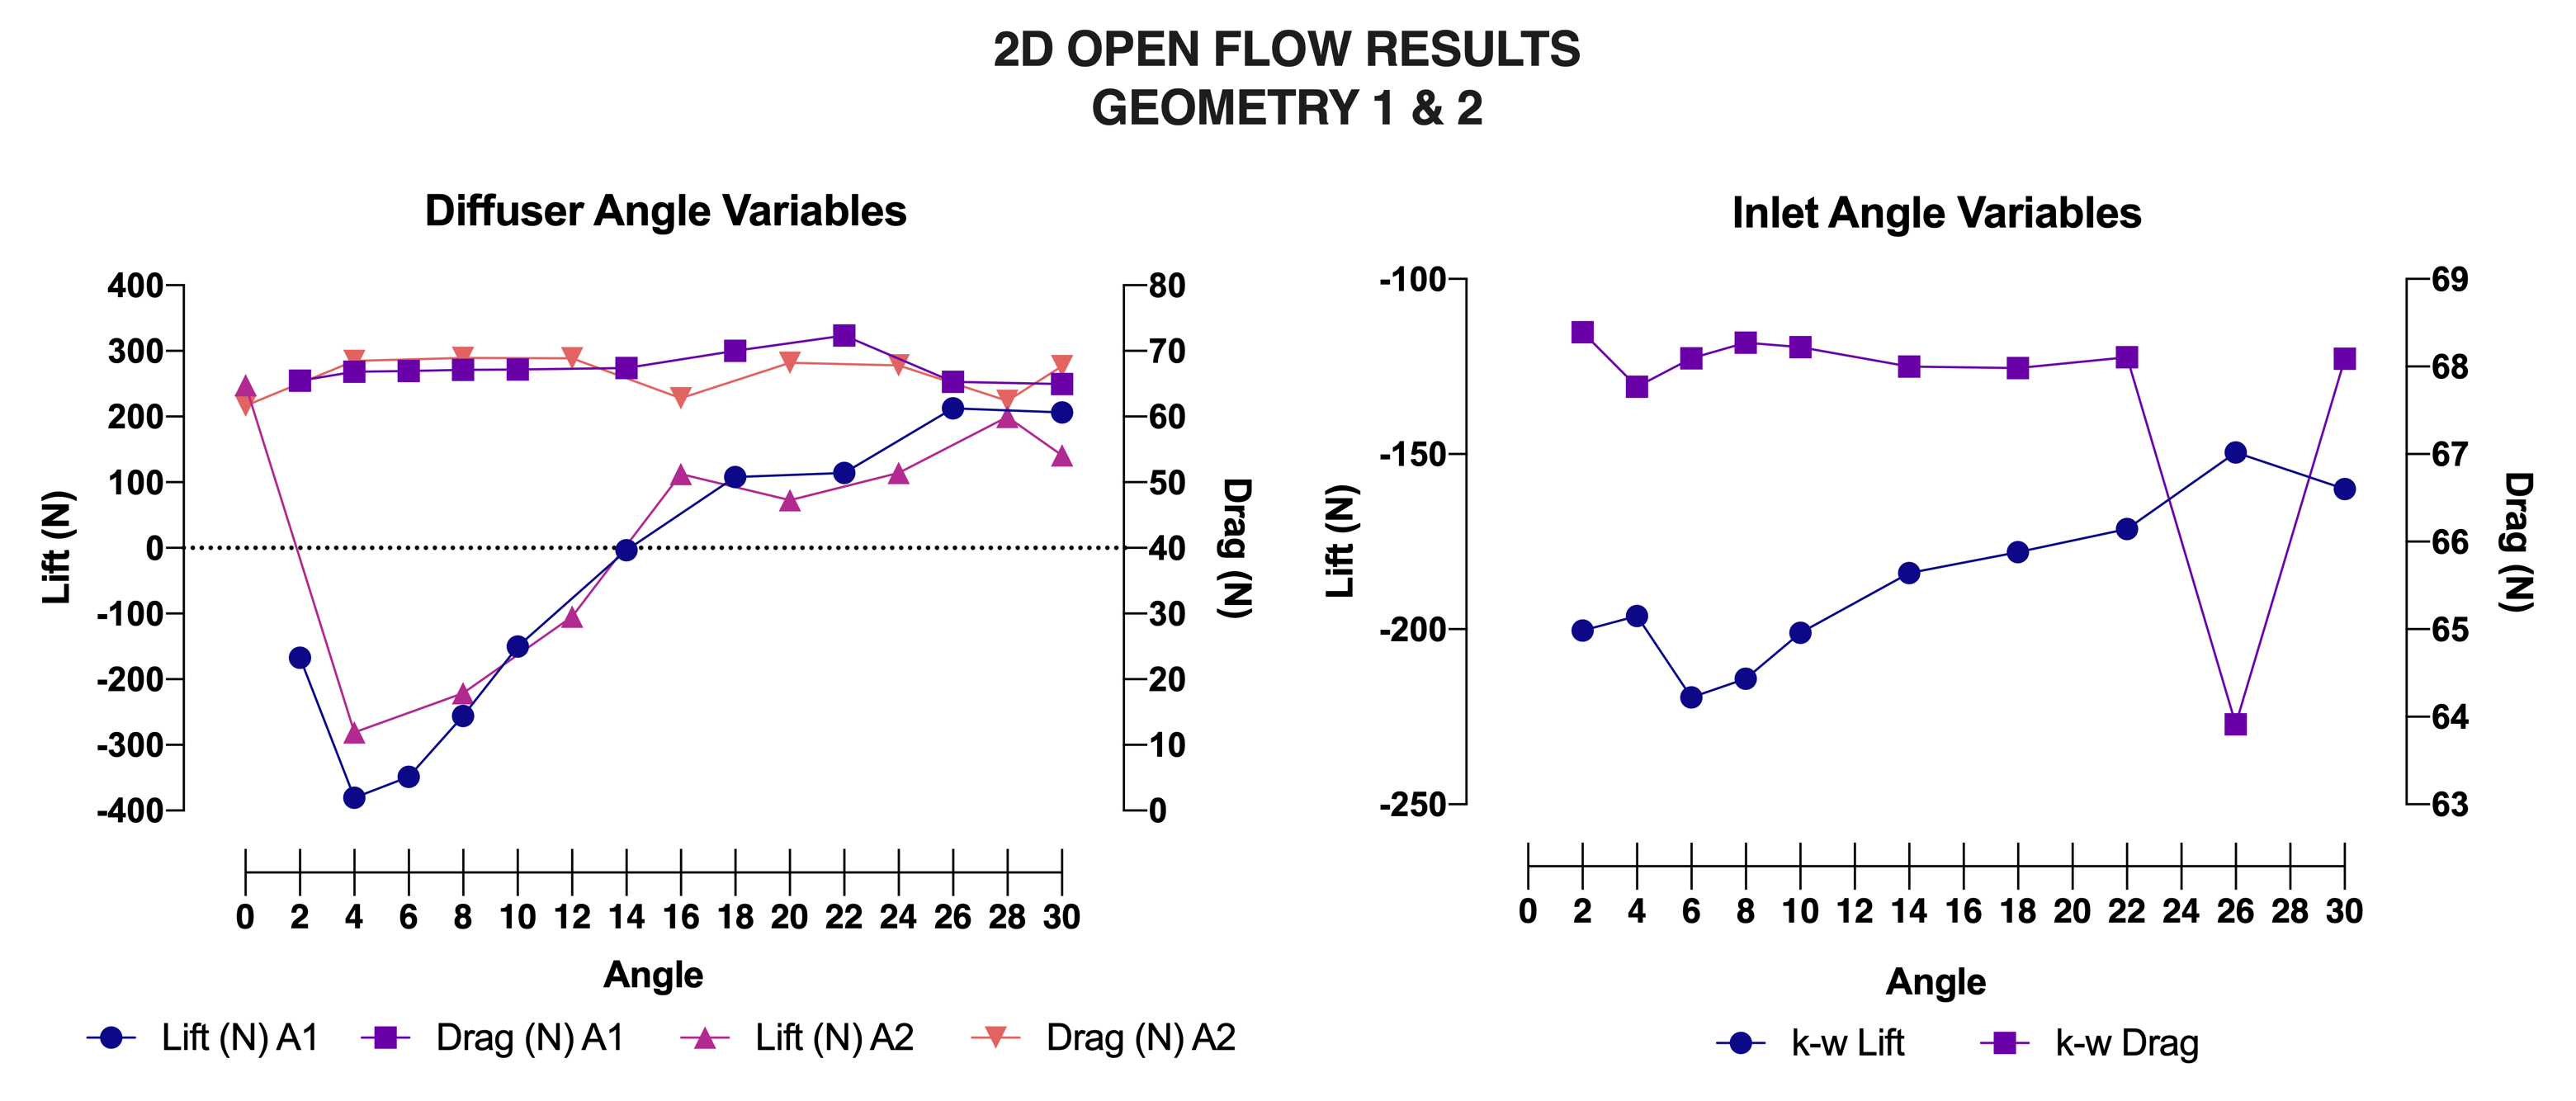
\includegraphics[scale = 0.65]{Figures/Graph/2D_OF_A1-2.png}
    \caption{Lift and drag variation plot of diffuser ange }
    \label{fig:2D_OF_A12_results}
\end{figure}







